\documentclass[11pt,a4paper]{article}

\usepackage[utf8]{inputenc}
\usepackage[ngerman]{babel}

\usepackage{amsmath}
\usepackage{amssymb}
\usepackage{mathtools}
\usepackage{xfrac}

\usepackage{xcolor}

\usepackage{enumerate}

\usepackage{fancyhdr}

\usepackage{graphicx}

\usepackage{listings}

\pagestyle{fancy}

\fancyhf[HR]{Lukas Vormwald, Noah Mehling, Gregor Seewald}
\fancyhf[HL]{Übung:Dienstag 14:00}

\title{Rechenanlagen\\Übungsblatt 5}
\author{Lukas Vormwald \and Noah Mehling \and Gregor Seewald}
\date{Übung :Dienstag 14:00}

\newcommand{\nor}[0]{\ensuremath{\text{ nor }}}

\DeclarePairedDelimiter\ceil{\lceil}{\rceil}
\DeclarePairedDelimiter\floor{\lfloor}{\rfloor}

\DeclarePairedDelimiter\abs{\lvert}{\rvert}%
\DeclarePairedDelimiter\norm{\lVert}{\rVert}%

% Swap the definition of \abs* and \norm*, so that \abs
% and \norm resizes the size of the brackets, and the
% starred version does not.
\makeatletter
\let\oldabs\abs
\def\abs{\@ifstar{\oldabs}{\oldabs*}}
%
\let\oldnorm\norm
\def\norm{\@ifstar{\oldnorm}{\oldnorm*}}
\makeatother

\begin{document}
\maketitle
  \section*{Aufgabe 5.1}
  \lstset{language=vhdl,keywordstyle=\color{blue}, numbers=left}
    \begin{lstlisting}
      ENTITY xnor IS
        PORT (x,y : IN bit; z : OUT bit)
      END xnor
      ARCHITECTURE behavior OF xnor IS
        CONSTANT tdhl : TIME := 25ps;
        CONSTANT tdlh : TIME := 45ps;
      BEGIN
        PROCESS(x,y)
        BEGIN
          IF x=y
            THEN z <= '1' AFTER tdlh;
            ELSE z <= '0' AFTER tdhl;
          END IF
        END PROCESS
      END behavior
    \end{lstlisting}

  \section*{Aufgabe 5.2}
    $\bar a \vee by$\\
    $\overline{(\overline{(\bar a \vee by)})}$\\
    $\overline{((a \bar b \vee \bar y))}$\\
    $\overline{(\bar a \nor \bar b \nor y)}$\\
    $\bar a \nor \bar b \nor y \nor \bar a \nor \bar b \nor y$\\
    $(a \nor a) \nor ((b \nor y) \nor (b \nor y)) \nor ((a \nor a) \nor ((b \nor y) \nor (b \nor y))$

\newpage

  \section*{Aufgabe 5.3}

  \begin{figure}[ht!]
    \centering
    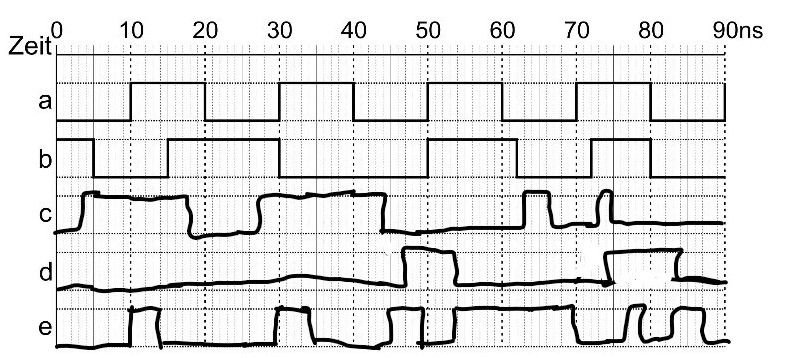
\includegraphics[width=126mm]{/home/gregor/grseewald.github.io/2_Semester/Rechenanlagen/Uebungen/5_3.jpg}
%    \caption{A simple caption \label{overflow}}
  \end{figure}

\end{document}
